\clearpage
\myparagraph{\olly}

\RU{Так как этот пример немного запутанный, попробуем оттрассировать его в}\EN{Since this example is tricky, 
let's trace it in} \olly.\\
\\
\olly \RU{может распознавать подобные switch()-конструкции, так что он добавляет полезные комментарии}\EN{can 
detect such switch() constructs, so its add some useful comments}.
\EAX \RU{в начале}\EN{is} $2$\EN{ at start}, \RU{это входное значение ф-ции}\EN{that's function's input value}: 

\begin{figure}[H]
\centering
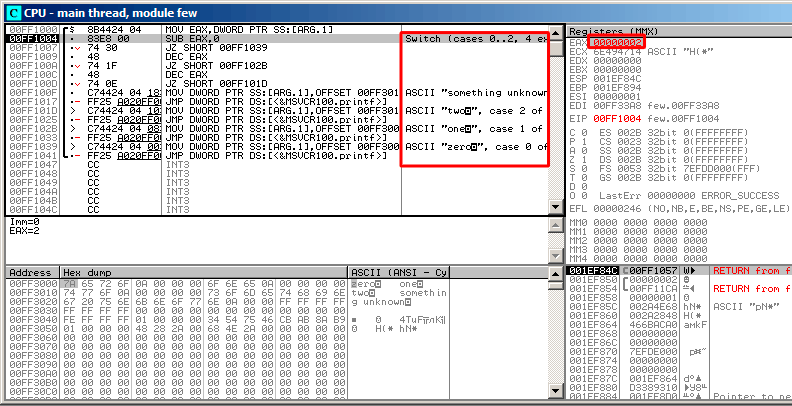
\includegraphics[scale=\FigScale]{patterns/08_switch/1_few/olly1.png}
\caption{\olly: \EAX \RU{содержит первый (и единственный) аргумент ф-ции}
\EN{now contain first (and sole) function argument}}
\label{fig:switch_few_olly1}
\end{figure}

\clearpage
$0$ \RU{отнимается от}\EN{is subtracted from} $2$ \InENRU \EAX. 
\RU{Конечно же}\EN{Of course}, \EAX \RU{все еще содержит}\EN{is still contain} $2$.
\RU{Но флаг}\EN{But} \ZF \RU{теперь}\EN{flag is now} $0$, \RU{что означает, что последнее вычисленное значение
не было нулевым}\EN{indicating that resulting value is non-zero}:

\begin{figure}[H]
\centering
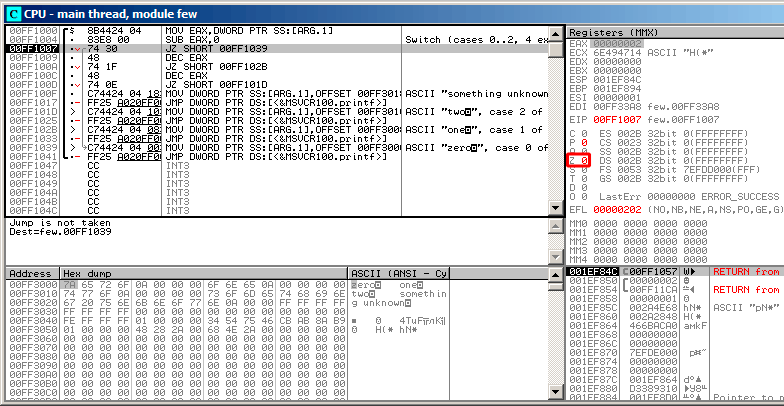
\includegraphics[scale=\FigScale]{patterns/08_switch/1_few/olly2.png}
\caption{\olly: \SUB \RU{исполнилась}\EN{executed}}
\label{fig:switch_few_olly2}
\end{figure}

\clearpage
\DEC \RU{исполнилась и}\EN{is executed and} \EAX \RU{теперь содержит}\EN{now contain} $1$. 
\RU{Но}\EN{But} $1$ \RU{не ноль, так что флаг}\EN{is non-zero, so the} \ZF \RU{все еще}\EN{flag is still} $0$:

\begin{figure}[H]
\centering
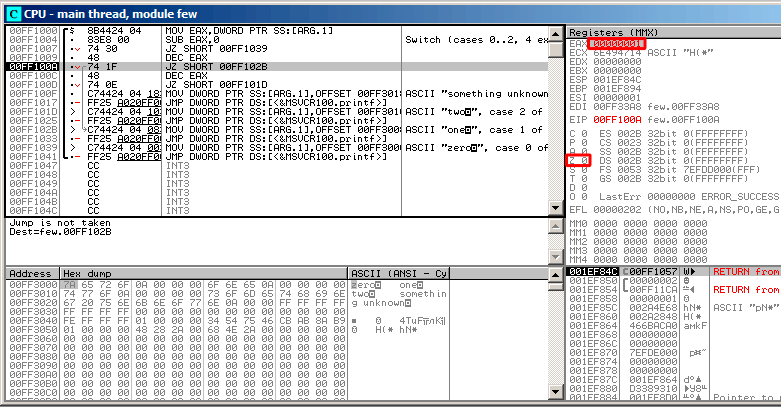
\includegraphics[scale=\FigScale]{patterns/08_switch/1_few/olly3.png}
\caption{\olly: \RU{первая}\EN{first} \DEC \RU{исполнилась}\EN{executed}}
\label{fig:switch_few_olly3}
\end{figure}

\clearpage
\RU{Следующая}\EN{Next} \DEC \RU{исполнилась}\EN{is executed}. 
\EAX \RU{наконец}\EN{is finally} $0$ \RU{и флаг}\EN{and} \ZF \RU{выставлен, потому что результат --- ноль}\EN{flag
is set, because the result is zero}:

\begin{figure}[H]
\centering
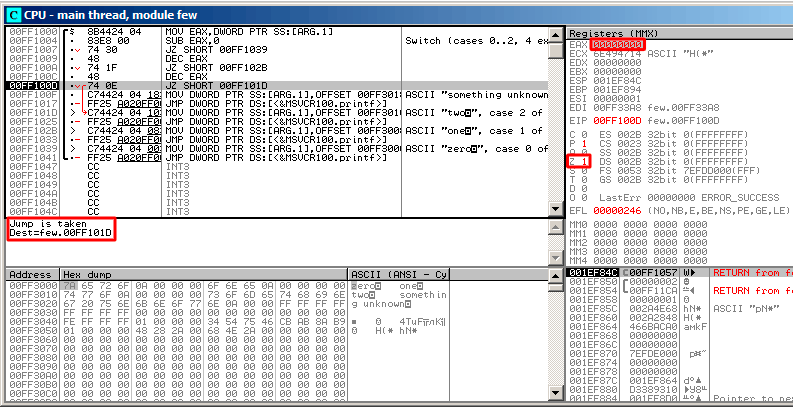
\includegraphics[scale=\FigScale]{patterns/08_switch/1_few/olly4.png}
\caption{\olly: \RU{вторая}\EN{second} \DEC \RU{исполнилась}\EN{executed}}
\label{fig:switch_few_olly4}
\end{figure}

\olly \RU{показывает, что условный переход сейчас сработает}\EN{shows that this jump will be taken now}.

\clearpage
\RU{Указатель на строку}\EN{A pointer to the string} ``two'' \RU{сейчас будет записан в стек}\EN{will now be 
written into the stack}:

\begin{figure}[H]
\centering
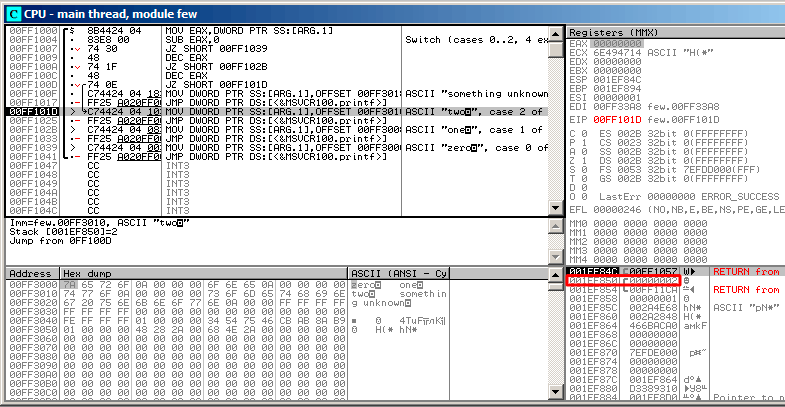
\includegraphics[scale=\FigScale]{patterns/08_switch/1_few/olly5.png}
\caption{\olly: \RU{указатель на строку сейчас запишется на место первого аргумента}
\EN{pointer to the string is to be written at the place of first argument}}
\label{fig:switch_few_olly5}
\end{figure}

\RU{Обратите внимание: текущий аргумент ф-ции это $2$ и $2$ прямо сейчас в стеке по адресу}\EN{Please note: 
current argument of the function is $2$ and $2$ is now in the stack at the address} \TT{0x0020FA44}.

\clearpage
\MOV \RU{записывает указатель на строку по адресу}\EN{wrote pointer to the string at the address} 
\TT{0x0020FA44} (\RU{см. окно стека}\EN{see stack window}).
\RU{Переход сработал}\EN{Jump is happen}.
\RU{Это самая первая инструкция ф-ции}\EN{This is the first instruction of} \printf \RU{в}\EN{function in} 
MSVCR100.DLL (\RU{я скомпилировал этот пример с опцией /MD}\EN{I compiled the example with /MD switch}): 

\begin{figure}[H]
\centering
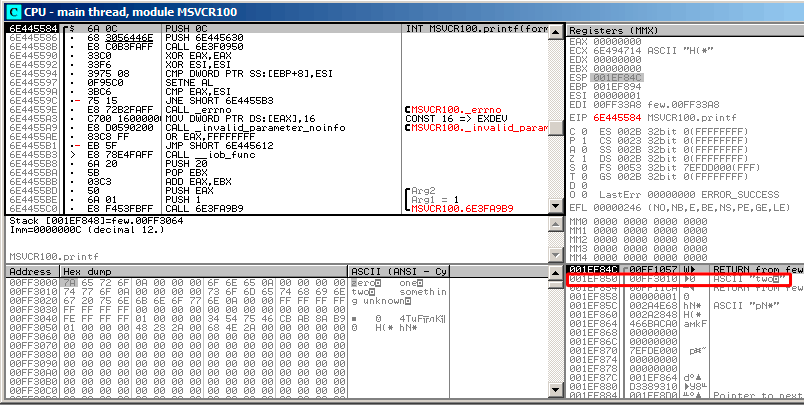
\includegraphics[scale=\FigScale]{patterns/08_switch/1_few/olly6.png}
\caption{\olly: \RU{первая инструкция в}\EN{first instruction of} \printf \InENRU MSVCR100.DLL}
\label{fig:switch_few_olly6}
\end{figure}

\RU{Теперь}\EN{Now the} \printf \RU{будет считать строку на}\EN{will treat the string at} \TT{0x00FF3010} 
\RU{как свой единственный аргумент и выведет строку}\EN{as its sole argument and will print the string}.

\clearpage
\RU{Это самая последняя инструкция ф-ции}\EN{This is the very last instruction of} \printf:

\begin{figure}[H]
\centering
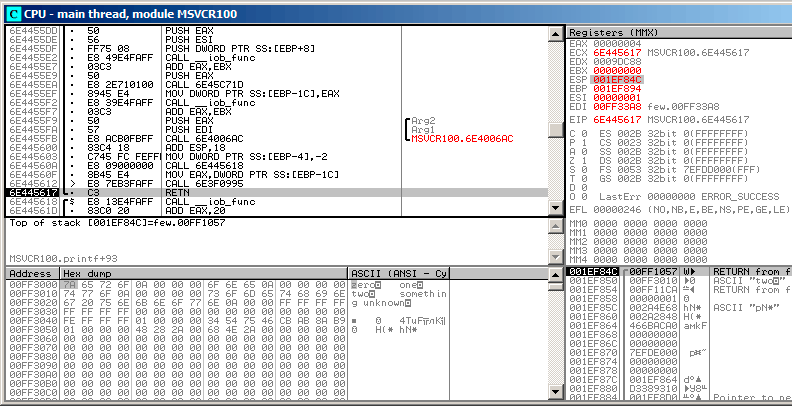
\includegraphics[scale=\FigScale]{patterns/08_switch/1_few/olly7.png}
\caption{\olly: \RU{последняя инструкция в}\EN{last instruction of} \printf \InENRU MSVCR100.DLL}
\label{fig:switch_few_olly7}
\end{figure}

\RU{Строка }``two'' \RU{была только что выведена в консоли}\EN{string was just printed to the console window}.

\clearpage
\RU{Нажмем}\EN{Let's press} F7 \OrENRU F8 (\stepover) \RU{и вернемся}\EN{and we will return}\dots
\RU{нет, не в ф-цию}\EN{not to} \ttf \RU{но в}\EN{function, but rather to the} \main:

\begin{figure}[H]
\centering
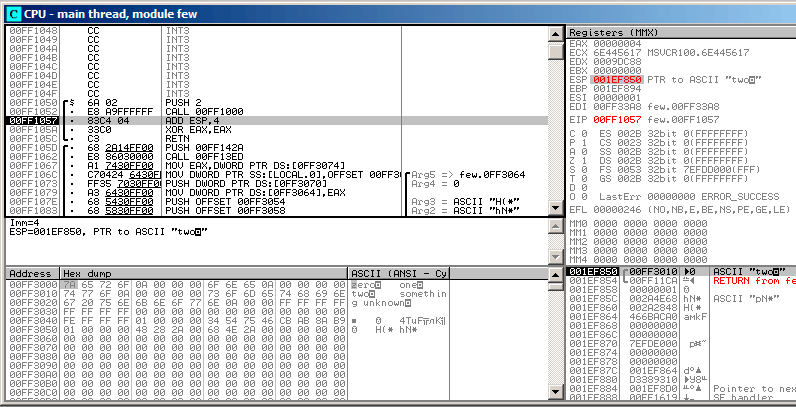
\includegraphics[scale=\FigScale]{patterns/08_switch/1_few/olly8.png}
\caption{\olly: \RU{возврат в}\EN{return to} \main}
\label{fig:switch_few_olly8}
\end{figure}

\RU{Да, это прямой переход из внутренностей}\EN{Yes, the jump was direct, from the guts of} \printf 
\RU{в}\EN{to} \main.
\RU{Потому как}\EN{Because} \ac{RA} \RU{в стеке указывает не на какое-то место в ф-ции}\EN{in the stack pointed 
not to some place in} \ttf \RU{а в}\EN{function, but rather to} \main.
\RU{И}\EN{And} \CALL \TT{0x00FF1000} \RU{это инструкция вызывающая ф-цию}\EN{was the actual instruction, which called} 
\ttf\EN{ function}.
